\section{Methodology}
\label{Methodology}
This thesis adopts a quantitative, simulation-based experimental research design, by comparing the designed Barrier Control algorithm against a baseline model, the FAS controller. The comparison is performed in an identical simulation environment in CARLA, which is chosen for its realistic vehicle dynamics \parencite{dosovitskiy2017carla}. The simulation environment consists of a closed-loop figure-eight track with a single intersection, where four traffic densities are tested across 30 independent runs each. The performance of the controllers is evaluated using four key performance indicators: throughput, delay time, energy consumption and number of near-crash collision violations. 
\\\\
The remainder of this chapter discusses the simulation environment, section~\ref{Sim environment}, the experimental conditions, section~\ref{Experimental Design}, and the measurement and validation approach, section~\ref{Key Performance Indicators},


 
\subsection{Simulation Environment}
This section describes the complete simulation environment by explaining the figure-eight map, the vehicle fleet, the vehicle controllers, and the energy model. 
\label{Sim environment}


\subsubsection{Figure-Eight Map and Distance Mapping}
\label{Figure-eight track}
The control strategies are evaluated in CARLA, in which a custom map is used, which is generated using Roadrunner. The evaluation is performed on a closed loop figure-eight, illustrated in figure~\ref{fig:figure8_combined}. The figure-eight ensures vehicles arrive at the intersection continuously and is generated using parametric equations, best described by equation~\ref{MAP}
\begin{equation}
\label{MAP}
    x(t) = -R\sin{t}, \ y(t) = -R\sin{2t}, \ t\in[0,2\pi],
\end{equation}
with radius \(R \)(m), and the position \(t\)(rad). The negative sign guarantees that the standard drive direction of AVs in CARLA is aligned with increasing values of \(t\). 
This parametric setup, results in a closed loop track with two loops of identical size, which intersect exactly in the middle at \(t = \pi\), which is the location of the intersection and also the point of conflict, which both barrier and FAS controller manage. Vehicles traverse this intersection from two sides, either at respectively \(t=\pi\) or \(t=0\) (equivalently \(t=2\pi\)). 
\begin{figure}[H]
    \centering
    % First Subfigure (Left)
    \begin{subfigure}[b]{0.48\linewidth}
        \centering
        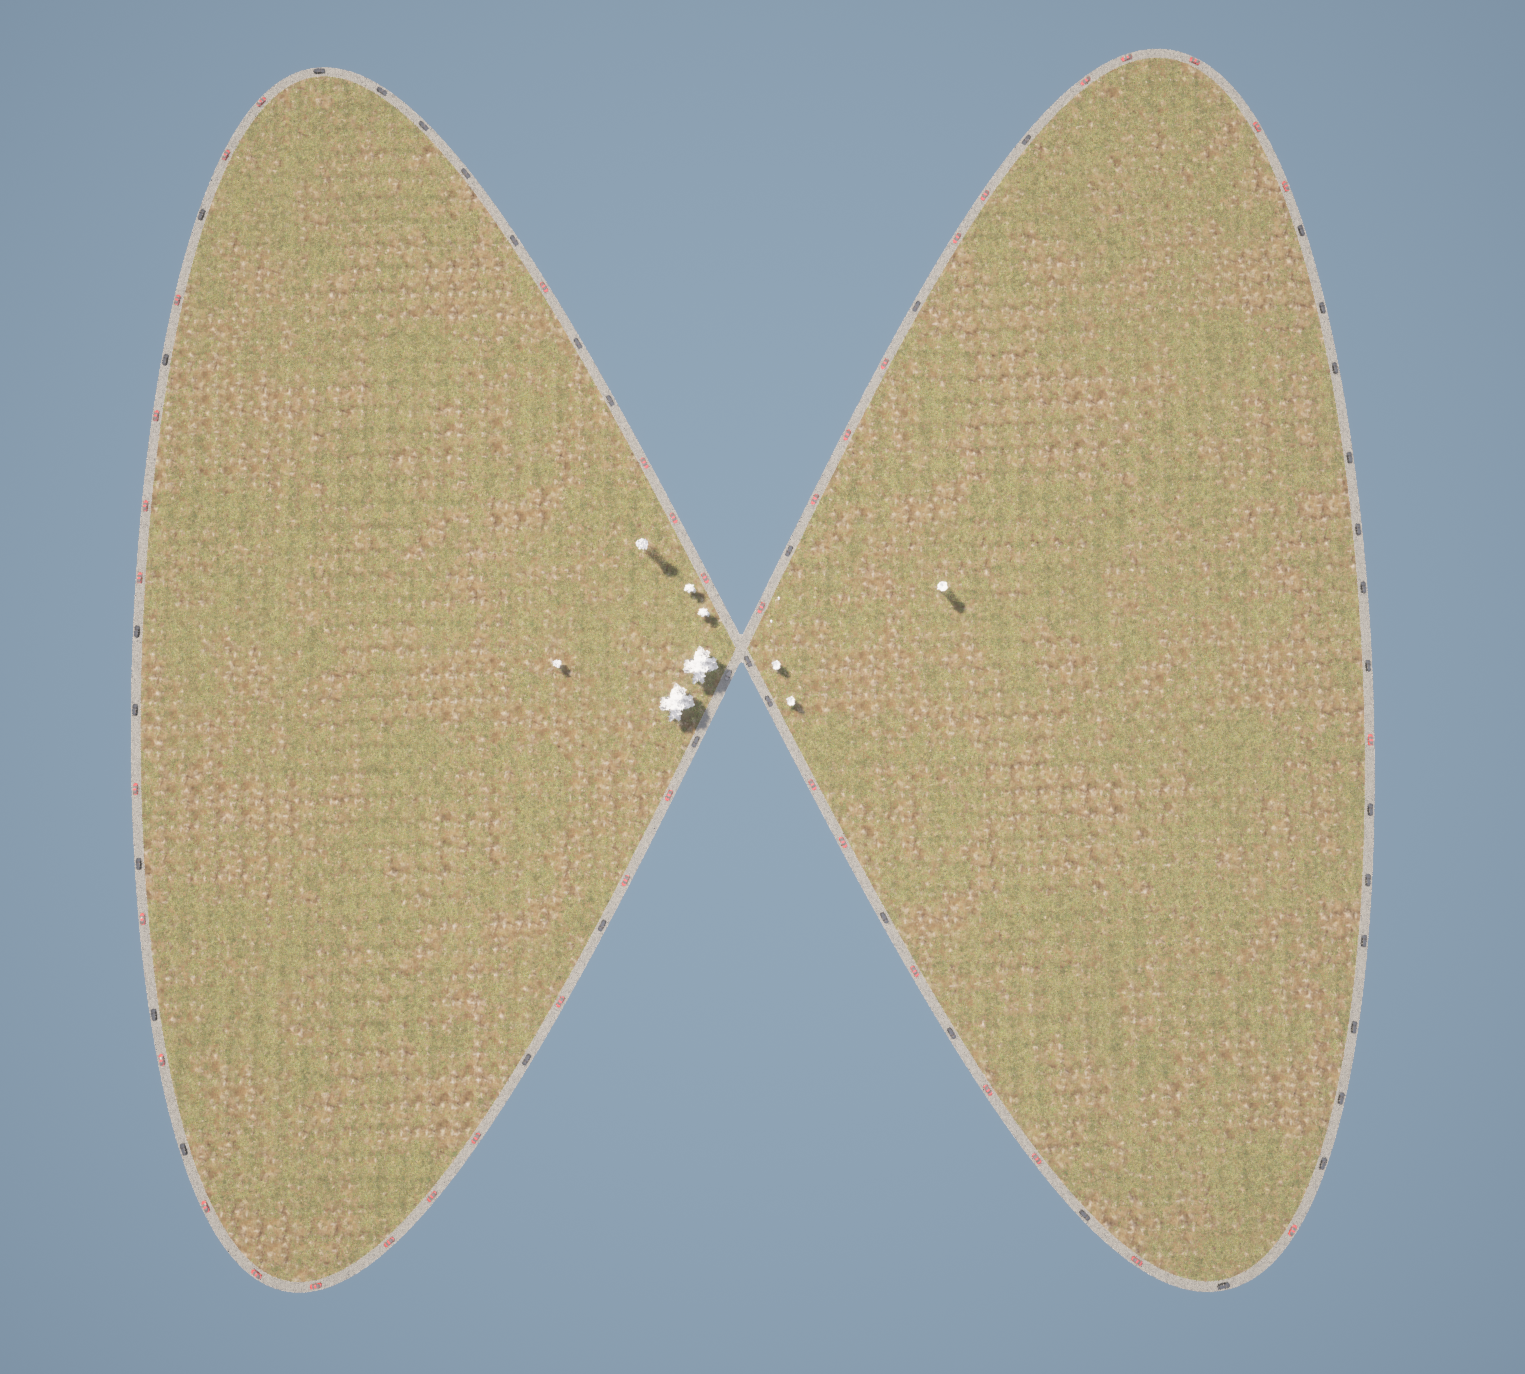
\includegraphics[width=\linewidth]{Screenshot from 2026-06-17 16-37-56.png}
        \caption{Overview of complete figure-eight}
        \label{fig:figure8_main}
    \end{subfigure}
    \hfill % Pushes the second subfigure to the right edge
    % Second Subfigure (Right)
    \begin{subfigure}[b]{0.48\linewidth}
        \centering
        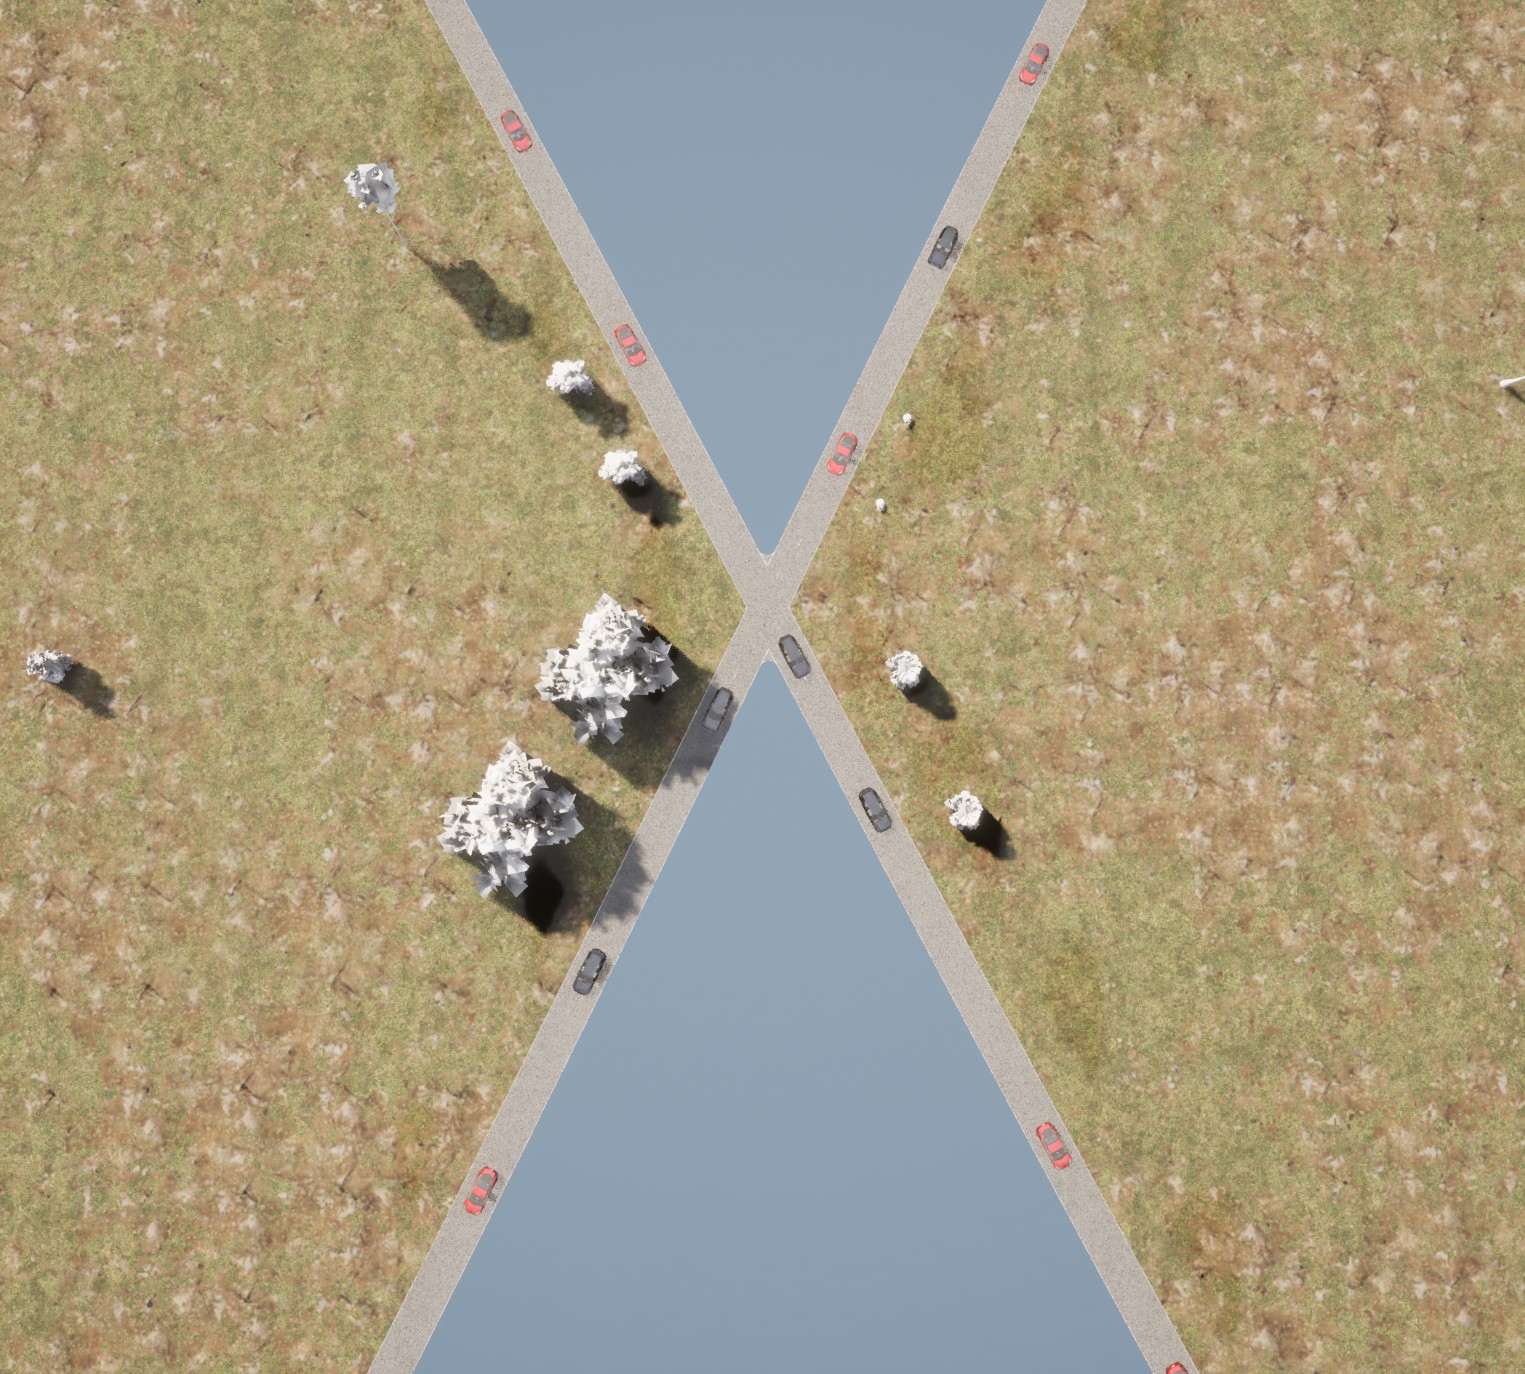
\includegraphics[width=\linewidth]{Screenshot from 2026-06-17 16-38-17.png}
        \caption{Figure-eight zoomed in at intersection}
        \label{fig:figure8_zoom}
    \end{subfigure}
    
    % Main Caption for the entire figure block
    \caption{Figure-eight Map: showing the complete map and a detailed close-up of the intersection with vehicles showing in red and black.}
    \label{fig:figure8_combined}
\end{figure}

On the figure-eight track, the position of an AV, is described by the parametric coordinate \(t\). However, the parametric coordinate is not suitable for the control strategies used in both simulations, since a difference between values of \(t\)  responds to the driven Euclidean distance. Nevertheless, the actual distance driven on the track is Geodesic. To resolve this issue, a distance mapper is used. At initialization, the distance mapper calculates the Arc Length \(L\)(m) using equation~\ref{arc length}
\begin{equation}
\label{arc length}
L =
\int_0^{2\pi}
\sqrt{
\left(\frac{dx}{dt}\right)^2 +
\left(\frac{dy}{dt}\right)^2
}
\,dt,
\end{equation} which is evaluated between 100000 equally spaced values of \(t\). The resolution of 100000 gives an accurate approximation of the true Geodesic distance by calculating the Euclidean distance of the small segments. The small segments are summed, and stored in a lookup table where each value of \(t\) corresponds to a geodesic distance \(s\)(m). Throughout the remainder of this chapter, linear interpolation is used to map from distance \(s\) to \(t\), section~\ref{Vehicle Fleet},  and from \(t\) to \(s\), section~\ref{Headway Control}.

\subsubsection{Vehicle Fleet and Initialization}
\label{Vehicle Fleet}
Two types of vehicles are used during the simulations, to reproduce a more realistic vehicle fleet. The vehicles used are the Tesla Model 3 RWD and the Audi e-tron 55, since these are listed in the standard CARLA vehicle library. Both vehicles differ in values with respect to weight \(m\)(kg), drag coefficient \(C_D\)(-), frontal area \(A_f(m^2)\), rolling resistance coefficient \(C_\text{rr}\)(-), gearbox ratio \(i_g\)(-), gearbox efficiency \(\eta_\text{gb}\)(-), wheel radius \(r_w\)(m), and motor efficiency \(\eta_\text{motor}\)(-). For the rolling resistance coefficient an average rolling resistance coefficient is used \parencite{swieczko2017tyre}. The gearbox efficiency value is assumed based on the typical efficiency of a planetary gearbox, which both vehicles use \parencite{lacock2023electric}. For motor efficiency, vehicle specific motor efficiency maps are used, which are extracted from current literature \parencite{rosenberger2024quantifying,thomas2021comparative} and shown in figure~\ref{fig:efficiency_contour}. The motor efficiency values are estimated using lookup tables, which are displayed in figure~\ref{fig:efficiency_lookups}. The remainder of the aforementioned values are displayed in table~\ref{vehicle specs}.

\begin{figure}[H] % 'htbp' is safer and more flexible than 'H'
    \centering
    % Subfigure A: Tesla Lookup
    \begin{subfigure}[b]{0.47\textwidth} % Slightly reduced width to safely fit margins
        \centering
        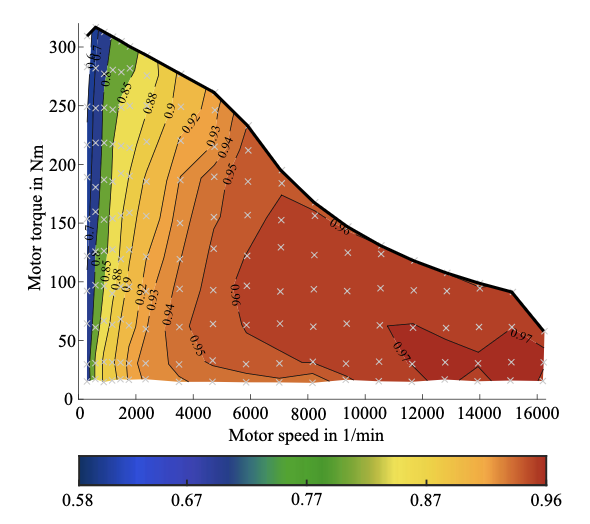
\includegraphics[width=\textwidth, height=4.5cm, keepaspectratio]{ContourTesla.png}
        \caption{Efficiency contour map of Tesla Model 3 RWD motor \parencite{rosenberger2024quantifying}.}
        \label{fig:tesla_lookup}
    \end{subfigure}% <-- This percent sign is CRITICAL. It prevents a hidden space.
    \hfill 
    % Subfigure B: Audi Lookup
    \begin{subfigure}[b]{0.47\textwidth}
        \centering
        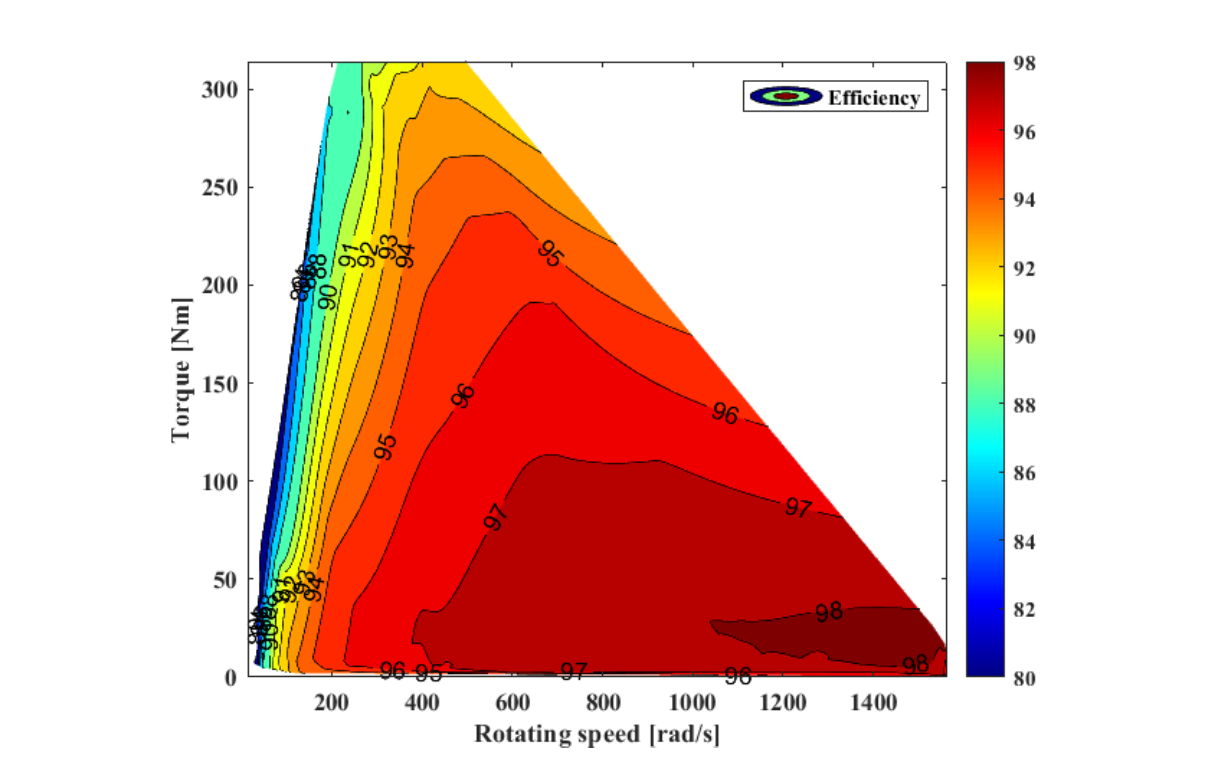
\includegraphics[width=\textwidth, height=4.5cm, keepaspectratio]{ContourAudi.png}
        \caption{Efficiency contour map of Audi e-tron 55 motor \parencite{thomas2021comparative}.}
        \label{fig:audi_lookup}
    \end{subfigure}
    
    \caption{Comparison of contour efficiency maps, Tesla Model 3 RWD vs. Audi e-tron 55.}
    \label{fig:efficiency_contour}
\end{figure}
\begin{figure}[H] % 'htbp' is safer and more flexible than 'H'
    \centering
    % Subfigure A: Tesla Lookup
    \begin{subfigure}[b]{0.47\textwidth} % Slightly reduced width to safely fit margins
        \centering
        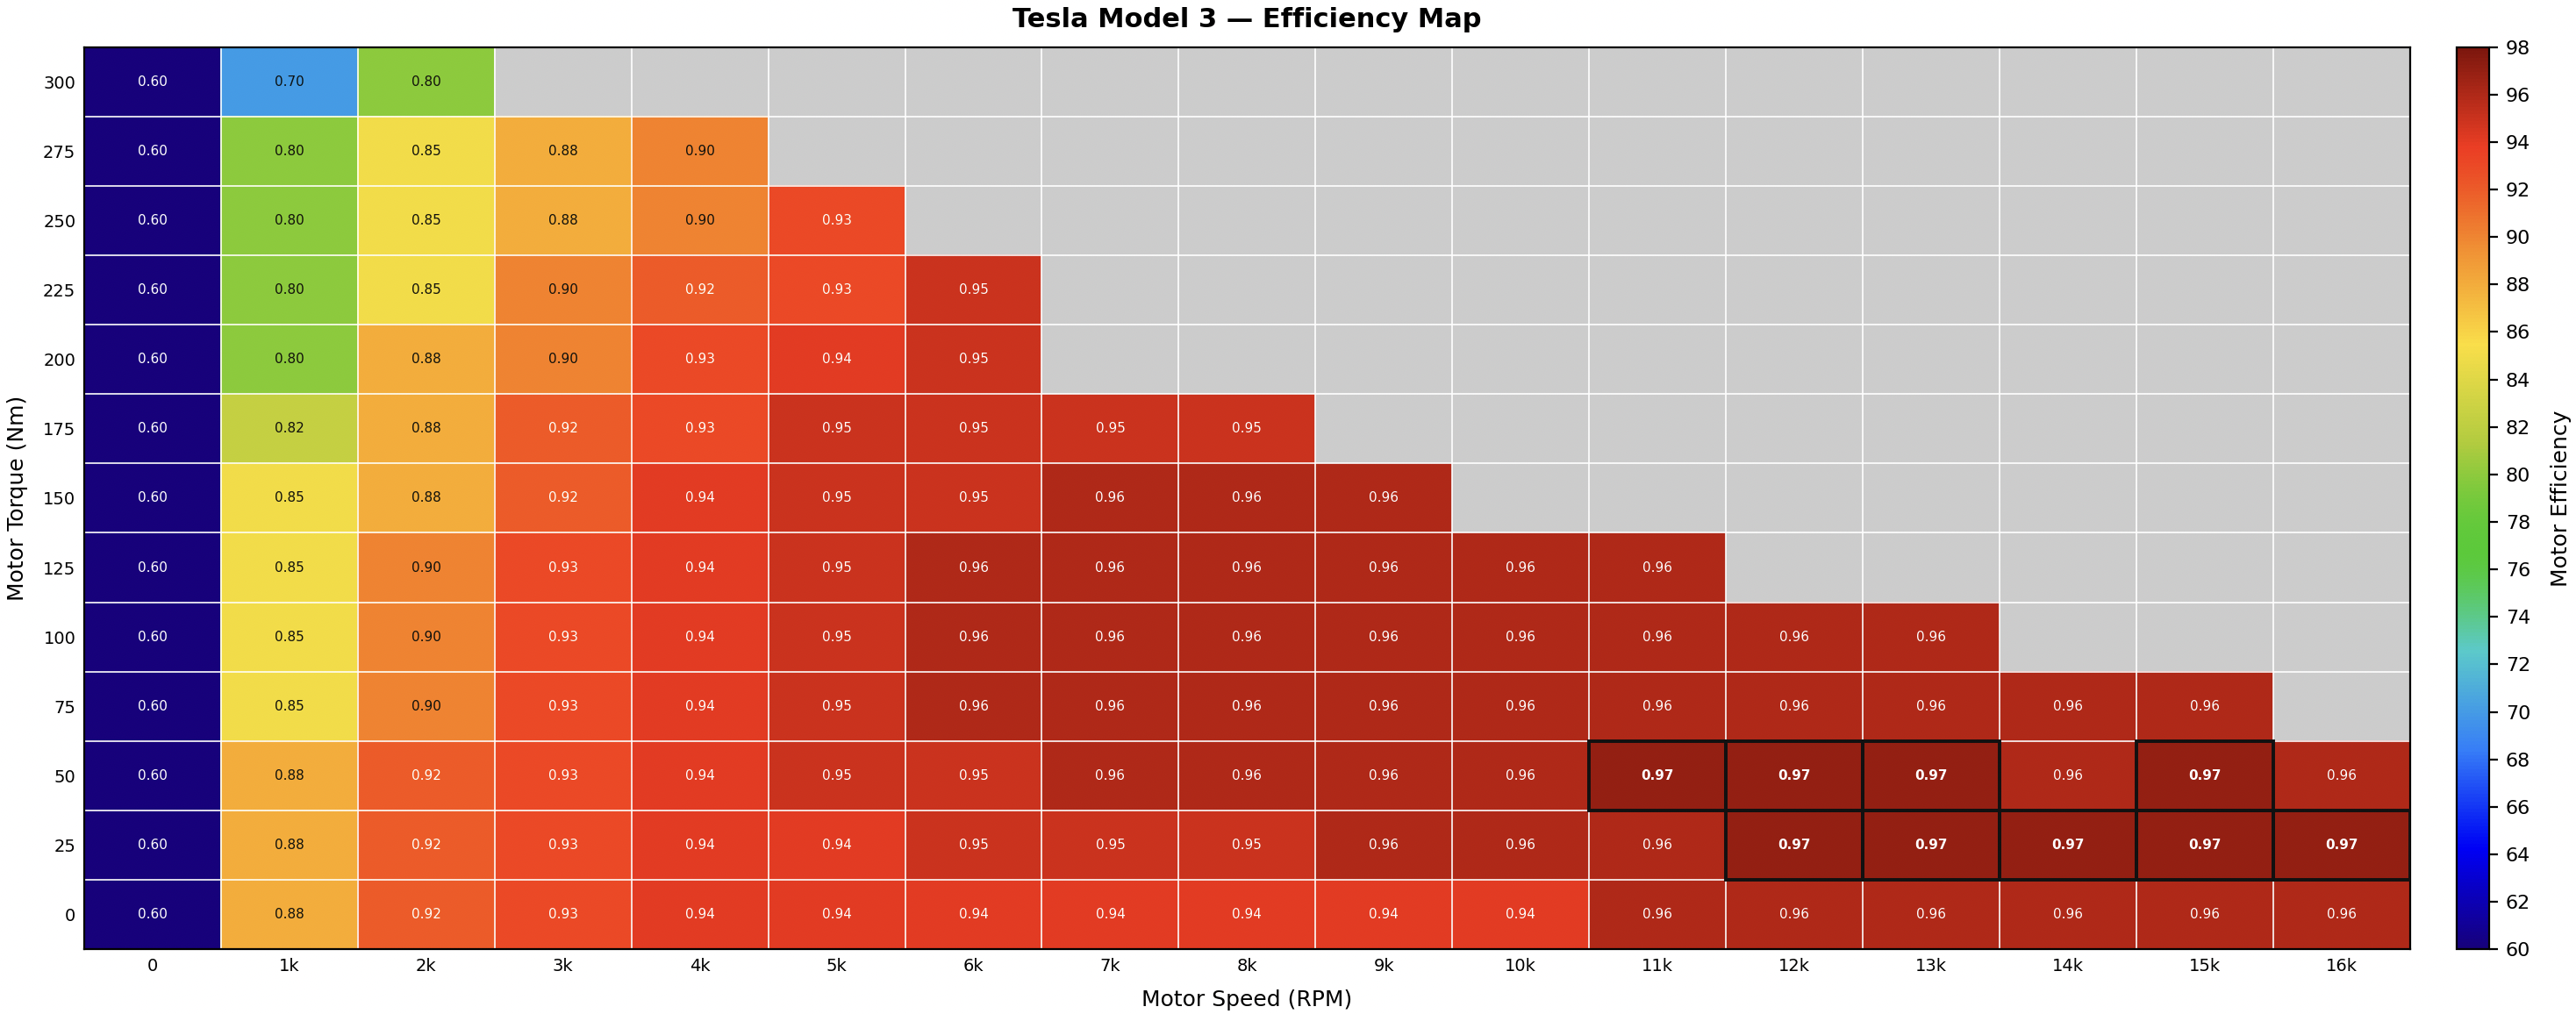
\includegraphics[width=\textwidth, height=4.5cm, keepaspectratio]{Table tesla.png}
        \caption{Lookup table of Tesla Model 3 RWD efficiency map}
        \label{fig:tesla_lookup}
    \end{subfigure}% <-- This percent sign is CRITICAL. It prevents a hidden space.
    \hfill 
    % Subfigure B: Audi Lookup
    \begin{subfigure}[b]{0.47\textwidth}
        \centering
        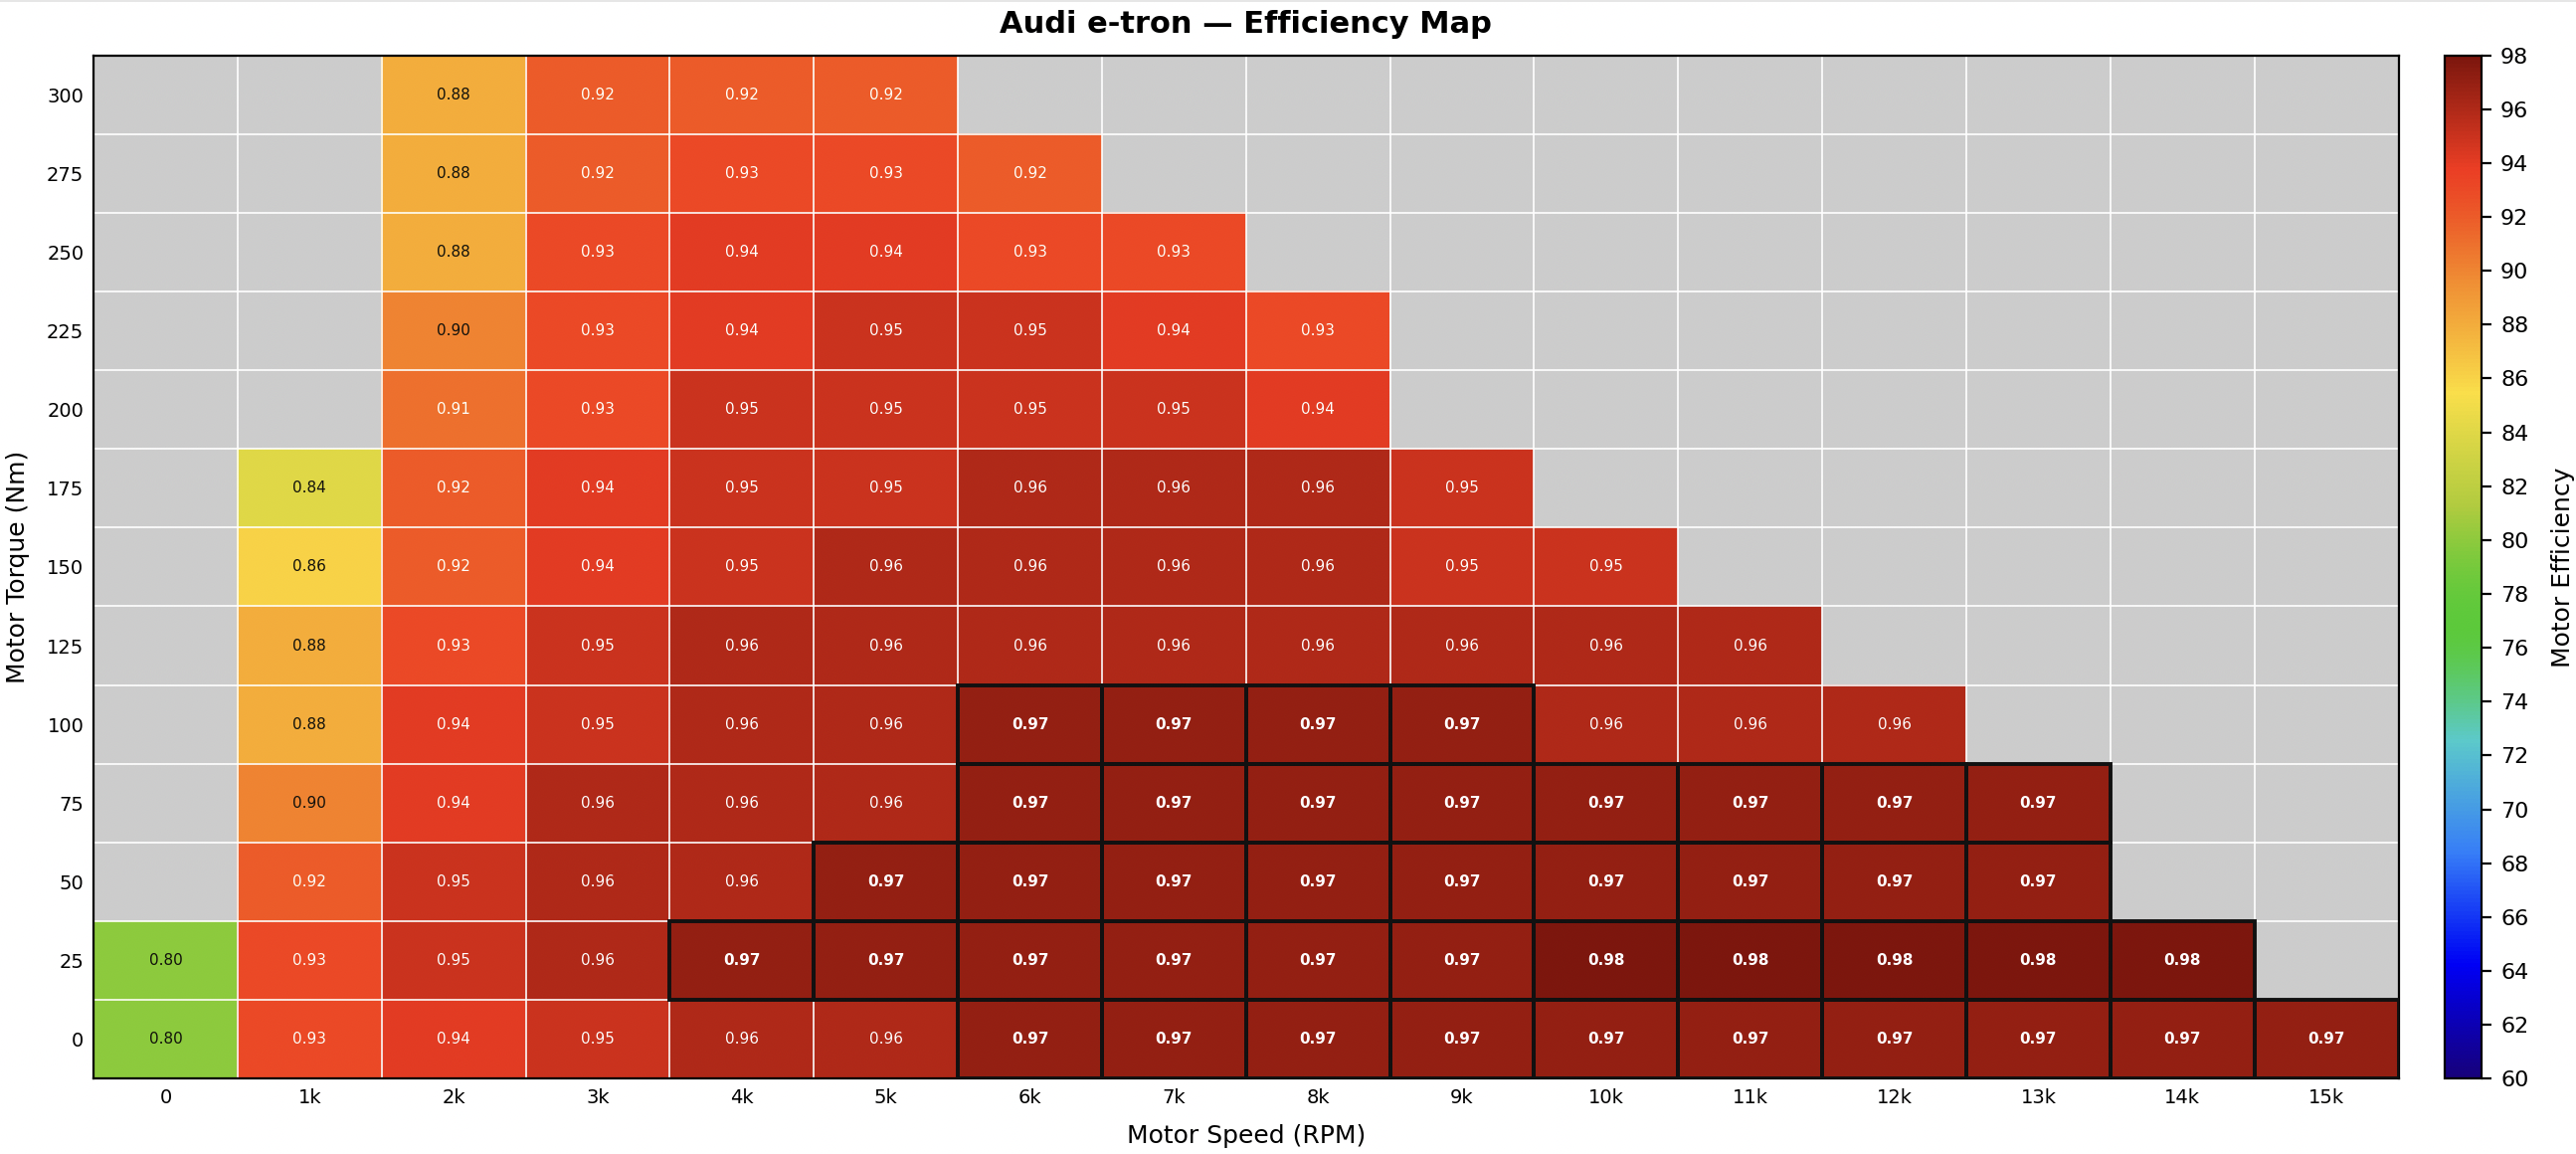
\includegraphics[width=\textwidth, height=4.5cm, keepaspectratio]{Table Audi.png}
        \caption{Lookup table of Audi e-tron 55 efficiency map}
        \label{fig:audi_lookup}
    \end{subfigure}
    
    \caption{Comparison of lookup tables generated from efficiency contour maps, Tesla Model 3 RWD vs. Audi e-tron 55.}
    \label{fig:efficiency_lookups}
\end{figure}

\begin{table}[H]
\centering
\caption{Per vehicle type specific parameters used during simulation: $^a$ sourced from manufacturer or press releases, $^b$ based on literature \parencite{swieczko2017tyre,rosenberger2024quantifying}, $^c$ assumed based on literature \parencite{lacock2023electric}.}
\begin{tabular}{lcc}

\toprule
\textbf{Parameter} & \textbf{Tesla Model 3 RWD} & \textbf{Audi e-tron 55} \\
\midrule
Weight, $m$ (kg) & 1931.0$^b$ & 2490.0$^a$ \\
Drag Coefficient, $C_D$ ($-$) & 0.23$^a$ & 0.28$^a$ \\
Frontal Area, $A_f$ ($\text{m}^2$) & 2.2$^a$ & 2.65$^a$ \\
Rolling Resistance Coeff., $C_{rr}$ ($-$) & 0.010$^b$ & 0.010$^b$ \\
Gearbox Ratio, $i_g$ ($-$) & 9.04:1$^b$ & 9.205:1$^a$ \\
Gearbox Efficiency, $\eta_{\text{gb}}$ ($-$) & 0.97$^c$ & 0.97$^c$ \\
Wheel Radius, $r_w$ (m) & 0.3468$^b$ & 0.3815$^a$ \\
\bottomrule
\end{tabular}
\label{vehicle specs}
\end{table}
With the vehicle types established, the vehicle initialization is started. Vehicle initialization consists of randomly spawning \(\frac{N}{2}+1\) Tesla Model 3s, and \(\frac{N}{2}\) Audi e-trons, with \(N\) the vehicle count, which is always an odd number. The placing of the vehicles starts each simulation run by placing the complete vehicle fleet \(N\) along the figure-eight track. The placement is performed using predefined target gaps \(d_\text{target}\) (m),  which is based on \(N\) and \(L\), and follows equation~\ref{Target} 
\begin{equation}
\label{Target}
    d_\text{target} = \frac{L}{N}.
\end{equation} The value of \(d_\text{target}\) is the input for the spawn positions of each vehicle along the track \(s_\text{target}\) (m), which follows equation~\ref{spawning}
\begin{equation}
\label{spawning}
    s_\text{target} = (j \times d_\text{target} + \epsilon\times d_\text{target}),
\end{equation}
with the vehicle number \(j\in\{1,N\}\), and the random spawn noise \(\epsilon\)(-). The computed spawn locations are linearly interpolated from \(s\) to \(t\), using the lookup table from section~\ref{Figure-eight track}, to align with the spawn approach used by CARLA. The value of \(t\) is compared to a list of safe spawn locations, which include all positions along the track except for the intersection. The intersection is excluded since two vehicles could spawn at the intersection at the same time, resulting in a direct crash during initialization. The vehicle, is therefore spawned at the safe spawn location which is closest to the value of \(t\) outside the intersection.

\subsubsection{Vehicle Controllers}
\label{Headway Control}
For driving along the track vehicles use a Headway Controller, which aims to maintain the target gap spacing between vehicles. The Headway controller adjusts based on the gap error \(e_\text{gap}(t)\)(m), between the target gap \(d_\text{t}\)(m), and the actual gap \(d_\text{actual}\)(m). \(d_\text{actual}\) corresponds to the Geodesic gap between the vehicle and its predecessor, which is derived using the lookup table generated by the Distance Mapper described in section~\ref{Figure-eight track}. This error is smoothed using an exponential moving average (EMA) filter, to account for a standard error between the math curve and the CARLA vehicle positions. 
\\\\
To adjust to errors in headway spacing, vehicles use a Proportional-Derivative (PD) controller, which takes \(e_\text{gap}(t)\) as input and computes a speed correction, \(u_\text{headway}\)(km/h), which follows equation~\ref{headwayeq}
\begin{equation}
\label{headwayeq}
    u_\text{headway}(t) = K_pe_\text{gap}(t)+ K_d\, \frac{d e_\text{gap}(t)}{dt},
\end{equation}
with the proportional gain \(K_p\ (km/h\cdot m)\) and the derivative gain \(K_d \ (km\cdot s/ m\cdot h)\). The speed correction is limited to ± 10 km/h, to ensure safe and comfortable control actions for vehicles in both simulations. Especially in the FAS simulation this limit is necessary, since the headway gap between a vehicle waiting on a red light, and its predecessor which just passed the red light, can grow very large. The large gap can result in a large headway error, which leads to a high speed correction demanded by the PD-controller, The high speed correction leads to maximum throttle when the light switches to green. Since this behavior is not aligned with realistic vehicle behavior at traffic lights, the limit of ±10 km/h is applied. 
\\\\
To respond to the various speed demands from the headway controller, barrier controller or vehicle response to the FAS controller, each vehicle uses a longitudinal controller. This controller, implemented as a Proportional-Integral-Derivative (PID) controller, translates the error between current speed and target speed,  \(e_\text{speed}(t)\), in various throttle and brake commands \(u_\text{throttle,brake}\), which follows equation~\ref{long}
\begin{equation}
\label{long}
    u_\text{throttle,brake} =  K_pe_\text{speed}(t)+ Ki \int_0^te_\text{speed}(\tau)d\tau + K_d\, \dot{e}_\text{speed}(t), 
\end{equation}
The \(u_\text{throttle,brake}\) commands are limited to ±1, where a command of +1.0 represents maximum throttle, and -1.0 represent maximum braking.  
\\\\
 Lastly, lateral control of the vehicles is handled by computing a look-ahead point on the track, which is done by advancing the current trajectory parameter \(t\) with a look-ahead step, which scales with the track radius, R. The steering is performed based on the signed angle between the vehicles current heading and the direction toward the look-ahead point. The output is bounded to ±1, which aligns with CARLAs steering input range.
\subsubsection{Energy Consumption Model}
\label{energy model explain}
The energy consumption model tracks the actual power drawn or restored from the battery during each simulation step, accounting for drivetrain losses in both directions. The battery power differs from the mechanical power delivered at the wheels during propulsion and regeneration. During propulsion efficiency losses in both motor and gearbox require more delivered battery power than the mechanical power at the wheels, whereas during regenerative braking not all recovered energy is completely restored into battery power, due to similar efficiency losses in the opposite direction. The calculation below therefore details how power consumed or restored at the wheels converts to actual battery power in three steps.  
\\\\
First, the total longitudinal force \(F_\text{total}\)(N)~\ref{Ftotal} acting on the wheels during driving is calculated, which consists of acceleration force \(F_\text{inertia}\)(N), aerodynamic drag force \(F_\text{aero}\)(N), and rolling resistance force \(F_\text{rolling}\)(N) \begin{equation}
\label{Ftotal}
    F_\text{total} = \underbrace{ma}_{F_\text{inertia}} + \underbrace{\tfrac{1}{2}\rho C_d A v^2}_{F_\text{aero}} + \underbrace{C_\text{rr}mg}_{F_\text{rolling}},
\end{equation} with acceleration \(a (m/s^2)\), air density \(\rho (kg/m^3)\), vehicle speed \(v\)(m/s), and gravitational acceleration \(g (m/s^2)\). The vehicle speed is directly extracted from the value reported by CARLA. However, CARLA does not report vehicle acceleration, therefore acceleration is computed from the finite difference of vehicle speed between each timestep. Since the calculation is found to be sensitive to simulation noise, the computed acceleration is smoothed using an EMA filter, using \(\alpha_\text{acceleration}\) listed in table~\ref{tab:simulation_parameters}. All other necessary values are extracted from table~\ref{vehicle specs}, and the values are selected based on the defined vehicle type, Tesla or Audi.
\\\\
Second, following equation~\ref{mech}, which multiplies total longitudinal force with velocity, the instantaneous mechanical power demand at the wheels is derived, which describes the power that must be delivered at the wheels at the specific moment 
\begin{equation}
\label{mech}
    P_\text{mech}= F_\text{total}\cdot v.
\end{equation}
In principle, the computed \(P_\text{mech}\) differs from the actual battery power demand \(P_\text{bat}\)(W), due to losses in the transmission and the electric motor during propulsion, and similar losses during regenerative braking \parencite{luin2019microsimulation}. To account for gearbox losses, a constant gearbox efficiency factor is used \(\eta_\text{gb}\) and for motor losses the vehicle specific motor efficiency \(\eta_\text{motor}\) is used. This motor efficiency is not a fixed value, as efficiency depends on motor shaft speed \(N_\text{motor}\)(RPM) and motor torque \(\tau_\text{motor}\)(Nm), which are derived from vehicle speed and \(F_\text{total}\). The motor shaft speed follows equation~\ref{shaft speed}
\begin{equation}
\label{shaft speed}
    N_\text{motor} = \frac{i_g\cdot v \cdot 60}{2 \cdot\pi\cdot r_w},
\end{equation}
and motor torque is dependent on propulsion or regenerative braking and follows equation~\ref{torque}
\\
\begin{equation}
\label{torque}
\tau_{\text{motor}} = \begin{cases} 
\displaystyle\frac{F_{\text{total} \, r_w}}{i_g \ \,\eta_\text{gb}} & \text{if } F_{\text{total}} \geq 0 \quad \text{(propulsion)} \\[2ex] 
\displaystyle\frac{F_{\text{total} \, r_w \, \eta_\text{gb}}}{i_g} & \text{if } F_{\text{total}} < 0 \quad \text{(regenerative braking)},
\end{cases}
\end{equation}
whereas during propulsion more motor torque is needed to overcome losses, and during regenerative braking, a smaller amount of torque is produced by the braking \parencite{luin2019microsimulation}.
\\\\
Third, the determined values, \(N_\text{motor}\) and \(\tau_\text{motor}\), are used to extract vehicle specific motor efficiency \(\eta_\text{motor}\), from a lookup table, from which a figure is shown in figure~\ref{fig:efficiency_lookups}. The efficiency value is estimated, by bilinear interpolation between the adjacent cells in the lookup table.  
The actual battery power demand is calculated using equation~\ref{Pbat}, which utilizes the derived \(\eta_\text{motor}\), \(\eta_\text{gb}\), and \(P_\text{mech}\) \parencite{chen2021review}, where the sign of \(P_\text{mech}\) illustrates propulsion or regenerative braking \begin{equation}
\label{Pbat}
P_{\text{bat}} = \begin{cases}
\displaystyle\frac{P_{\text{mech}}}{\eta_\text{gb}\,\eta_\text{motor}} & \text{if } P_{\text{mech}} \geq 0 \quad \text{(propulsion)} \\[2ex]
P_{\text{mech}} \cdot \eta_\text{gb}\,\eta_\text{motor} & \text{if } P_{\text{mech}} < 0 \quad \text{(regenerative braking)}
\end{cases}.
\end{equation}
During propulsion, \(P_\text{mech}\) is divided by \(\eta_\text{gb}\) and \(\eta_\text{motor}\), to reflect the additional power drawn from the battery to overcome the losses. On the other hand, during braking, the power is multiplied with \(\eta_\text{gb}\) and \(\eta_\text{motor}\), which reflects the fraction of power actually regenerated to the battery due to regenerative braking \parencite{luin2019microsimulation}.
\\\\
This energy consumption model uses a few simplifying assumptions. First, since the figure-eight is flat, no gradient force is considered. Second, the motor efficiency maps are estimates from other researchers, due to limited availability of vehicle specific maps. Third, the Audi e-tron efficiency map excludes inverter efficiency, whereas the Tesla Model 3 map includes the inverter efficiency. Since no inverter efficiency coefficient could be found for the Audi e-tron, the inverter inefficiency is neglected, and therefore the efficiency of the Audi e-tron is being overestimated. Fourth, efficiency maps had empty regions, which are assumed to have low efficiency of 0.60. Fifth, the motor is assumed to be equally efficient during propulsion and regenerative braking. Finally, auxiliary loads, like heating, ventilation, and air conditioning are neglected, since it is a constant across both simulations. However, since all the assumptions influence both simulations identically, they do not affect the relative comparison.

\subsection{Experimental Design and Parameters}
\label{Experimental Design}
The barrier and FAS controller  are evaluated under identical conditions using the simulation framework~\ref{Sim environment}. This section describes how stochastic initial conditions were used across both controllers to evaluate robustness of the results.
\subsubsection{Traffic Density and Vehicle Initialization}
\label{Experimental setup}
To analyze the performance of both intersection control strategies under varying traffic density, four vehicle counts are evaluated: \(N \in\{51,61, 71, 81\}.\) To account for variability in initial conditions, each vehicle count is simulated over 30 independent simulation runs with spawn noise \(\epsilon\) of up to ±20 \%. The spawning follows formula~\ref{spawning} and an example of spawning with noise is displayed in figure~\ref{fig:figure8_zoom}. To ensure that any observed difference in KPIs can solely be attributed to the intersection management strategy, each simulation run uses a reproducible random seed which ensures that run \(k\) of the barrier controller uses identical conditions as run \( k\) of the FAS controller. 
\subsubsection{Simulation Phases and Parameters}
Simulations are performed using synchronous mode at a fixed timestep of \(\Delta t\)(s). This combination allows for precision between simulations and limits computational costs. With \(\Delta t\) in place, the simulation starts with a warm-up phase, during this phase vehicles are held stationary with the handbrake active, this is done to ensure that CARLA can spawn the vehicles correctly.  Next, a ramp-up phase starts, during this phase vehicles ramp-up to the target speed. During this phase the headway correction \(u_\text{headway}\), discussed in section~\ref{Headway Control}, is inactive, but both intersection management strategies are active to prevent collisions at the intersection during ramp-up. After the ramp-up phase, the evaluation-phase begins in which the headway controller also takes action. The durations of each phase and the simulation conditions are summarized in table~\ref{tab:sim_params}.
\\\\


\begin{table}[H]
\caption{Parameters used during all simulations }
\centering
\begin{tabular}{ll}
\toprule
\textbf{Parameter} & \textbf{Value} \\
\midrule
Simulation Time & 1800 s \\
Track Length (\(L\)) & 2347.4 m \\
Timestep (\(\Delta t\)) & 0.05 s \\
Warm-up Phase & 5 s \\
Ramp-up Phase & 12.5 s \\
Target Speed (\(v^*\)) & 30 km/h \\
Vehicle Counts ($N$) & 51, 61, 71, 81 \\
Spawn Noise (\(\epsilon\)) & $\pm$0.20\\
Runs per $N$ & 30 \\

\bottomrule
\end{tabular}

\label{tab:sim_params}
\end{table}




\subsection{Performance Measurement and Validation}
\label{Key Performance Indicators}
During the simulations, four KPIs are recorded. These KPIs form the basis for the quantitative analysis. The remainder of this section explains the key performance indicators and the validation approach.

\subsubsection{Throughput, Delay, Energy, and Safety Violations}
Throughput is measured as the number of vehicles that cross the intersection per unit of time \parencite{soltani2025communication}. In the simulation environment, vehicles can cross the conflict point from two sides, either halfway at \(t=\pi\) or at the wraparound point \(t = 0 \) (equivalently \(t=2\pi\)). A crossing is counted if a vehicle passes the conflict point. The total throughput rate \(I\)(veh/s), is the total number of crossings \(N_c\)(veh), divided by the elapsed time \(T\), which follows equation~\ref{throughput}
\begin{equation}
\label{throughput}
I = \frac{N_\text{c}}{T}.   
\end{equation}  
\\\\
Delay time is commonly measured in traffic studies to evaluate efficiency of intersection management systems \parencite{soltani2025communication}. It demonstrates the extra time it takes to traverse the intersection compared to a free flow situation. To compute delay time, the lap times of vehicles are calculated. To ensure that no delay occurs from the warm-up and ramp-up phase, the counting starts after completion of the two phases. After completion, the position of each vehicle is captured and stored. If the corresponding vehicle crosses its stored position again, it has completed a lap and the lap time is recorded. 
For calculating the per vehicle delay time \(t_\text{delay}\)(s), a free flow lap time is calculated. This lap time is found by simulating a complete lap, with only one vehicle, moving at the target speed. From the free flow lap time  \(t_\text{delay}\) can be calculated, which follows equation~\ref{Delay}
\begin{equation}
\label{Delay}
    t_\text{delay} = t_\text{actual}-t_\text{ideal},
\end{equation}
with the actual lap time \(t_\text{actual}\)(s), and the free flow lap time \(t_\text{ideal}\)(s). To find the per simulation delay, all values of \(t_\text{delay}\) are accumulated into total delay.
\\\\
Energy consumption is measured as the total battery power of all vehicles during a simulation run. For calculation, the per vehicle energy model described in section~\ref{energy model explain} is used. The per vehicle battery power is accumulated over time \parencite{chen2021review}, which follows~\ref{energy} \begin{equation}
\label{energy}
    E_\text{total} = \frac{1}{3.6\times10^6}\int_0^T P_\text{bat}dt, 
\end{equation} where \(\frac{1}{3.6\times10^6}\) is used to convert from J to kWh.
\\\\
The amount of safety violations is evaluated as the number of near-crash collisions at the intersection. A near-crash collision occurs if two simultaneously approaching vehicles from opposing sides cross within a predefined safety distance of each other. If the actual gap at the intersection falls below the predefined threshold value, a near-crash collision is counted.  The number of safety violations \(N_v\)(violations), is accumulated during simulation and divided by the elapsed time T(s) to get the safety violation rate S (violations/s), which follows equation~\ref{Safetyviolationseq}
\begin{equation}
\label{Safetyviolationseq}
       S = \frac{ N_v}{T}.
\end{equation}




\subsubsection{Validation Approach}
\label{System Validation}
To ensure the simulation framework produces reliable and realistic results, two validation steps are performed after the experiments.
\\\\
First, the headway controller is validated by verifying convergence to the target spacing during the evaluation phase for the barrier controller. Convergence is considered successful when all vehicles maintain a gap within 2.5 m from the target spacing. This validation is performed by manually comparing the target headway spacing to the actual headway spacing. In addition, a plot of both of the aforementioned parameters is created and manually inspected after each run.    
\\\\
Second, the four KPIs are validated. Throughput is validated by manual inspection and comparison to the theoretical maximum. The theoretical maximum is calculated based on the number of vehicles, the length of the track, and the target speed. The simulated throughput value is verified to remain within this theoretical maximum across all runs. A similar approach is used to validate delay time. The approach consists of a comparison of the actual lap time to the theoretical minimum, which is calculated from the length of the track and the target speed. Validation of the energy consumption model is done by comparing output of the simulations with publicly available energy consumption figures. The validation is performed to confirm that the power demand model produces realistic values. Lastly, the safety violations are validated by manual inspecting the violation measurement during simulations. 
\\\\








